\chapter{Introduction and Motivation}

In times of climate change, the need to reduce carbon emissions is prevalent. 
One area of interest is carbon produced via electrical power used in data centers. 
However, not all power is produced equally: while a data center may source its power from the public grid, the public grid itself is sourced from different producers. 
These include high-carbon intensive technologies such as coal and gas but also include low-carbon sources such as solar and wind. 
The latter, renewables and especially solar, follow a diurnal rhythm over the day as shown in Figure \ref{fig:energy_mix}.

\begin{figure}
    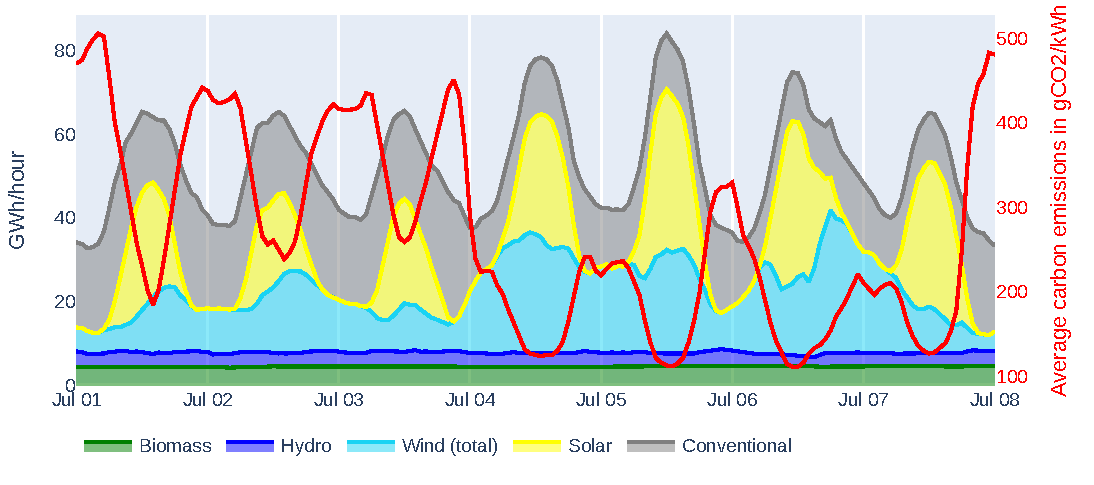
\includegraphics[width=\linewidth]{agorameter/energy_production_week.pdf}
    \caption[short]{Mix of energy production in Germany for the first week of July 2024\webcite{web_agora}}
    \label{fig:energy_mix}
\end{figure}

As the sun shines more during the day, a bigger part of the total power production then comes from solar, reducing the overall carbon intensity of the grid.
This can be used for \emph{carbon aware scheduling}, by planning work in datacenters to be executed during such low intensity times, the overall carbon can be reduced.

Data centers are currently projected to experience exponential growth in their power requirements, largely fueled by pushes in AI.\cite{schwartz_green_2019}

Current work on carbon aware scheduling includes shifting jobs temporally and spatially. 
One common theme among them, however, is that the workload models do not include program heterogeneity: while real world programs may include high-powered times for computation and low-powered times for e.g. I/O, this is not reflected in literature. 
Another common strategy for executing jobs during low-carbon timeframes, is to \emph{suspend \& resume}: a job may be, for example, stopped as carbon-intensity is increasing and resumed when a certain threshold is reached. 
This generally assumes, that resuming a job carries no overhead. 

In this work, we will improve upon the homogeneous, no overhead workload model used in literature, by measuring an AI program and deferring a new model upon that.

The research question will be the following:

\begin{enumerate}
    \item How high are carbon savings under a workload model including resume-overhead and power-heterogeneity?
    \item How does this compare to previous work in the field using the homogeneous model?
    \item Which jobs are better suited for carbon aware scheduling?
\end{enumerate}
